\clearpage
\section{Anexos}
\begin{longtable}{>{\raggedright\arraybackslash}p{5cm}>{\raggedright\arraybackslash}p{5cm}>{\raggedright\arraybackslash}p{5cm}}
    \caption{Matriz de consistencia.} \label{tab:preguntas_objetivos_hipotesis} \\
    \hline
    \textbf{PREGUNTA GENERAL} & \textbf{OBJETIVO GENERAL} & \textbf{HIPÓTESIS GENERAL} \\
    \hline
    \endfirsthead 
    \caption[]{(continuación)} \\
    \hline
    \textbf{Preguntas Específicas} & \textbf{Objetivos Específicos} & \textbf{Hipótesis Específicas} \\
    \hline
    \endhead
    \hline
    \multicolumn{3}{r}{\textit{Continúa en la siguiente página ...}} \\
    \endfoot
    \hline
    \endlastfoot
    ¿Es posible desarrollar un modelo de aprendizaje ensamblado para la detección de quema de caña de azúcar? & Desarrollar un modelo de aprendizaje ensamblado para la detección de quema de caña de azúcar a fin de mejorar su fiscalización. & El modelo de aprendizaje ensamblado para la detección de quema de caña de azúcar permitirá resultados con un gran porcentaje de efectividad. \\
    \hline
    \textbf{Preguntas Específicas} & \textbf{Objetivos Específicos} & \textbf{Hipótesis Específicas} \\
    \hline
    ¿Cómo generar el conjunto de datos necesario para el funcionamiento del modelo de aprendizaje ensamblado para detectar la quema de caña de azúcar? & Generar el conjunto de datos necesario para el funcionamiento del modelo de aprendizaje ensamblado para detectar la quema de caña de azúcar. & La correcta generación del conjunto de datos necesario para el funcionamiento del modelo de aprendizaje ensamblado para detectar la quema de caña de azúcar optimizará la precisión del modelo. \\
    ¿Cuáles son los algoritmos que mejor se ensamblan al modelo para detectar la quema de caña de azúcar? & Determinar los algoritmos que mejor se ensamblan al modelo para detectar la quema de caña de azúcar. & Los algoritmos LightGBM y U-Net serán los que mejor se ensamblan al modelo para detectar la quema de caña de azúcar. \\
    ¿El modelo de aprendizaje ensamblado presenta un desempeño superior en comparación con los algoritmos individuales? & Determinar mediante métricas de evaluación si el modelo de aprendizaje ensamblado presenta un desempeño superior en comparación con los algoritmos individuales. & El modelo de aprendizaje ensamblado presentará un desempeño superior en comparación con los algoritmos individuales. \\
    \hline
\end{longtable}

\begin{figure}[H]
    \centering
    \caption{Resumen de las ROI's.}
    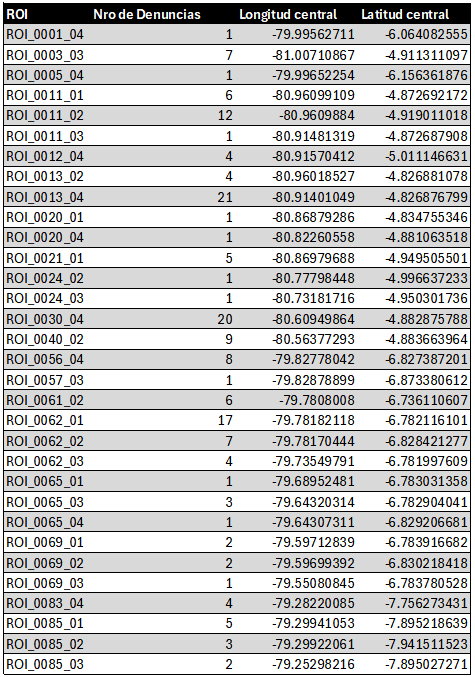
\includegraphics[width=0.9\textwidth]{img/8_capitulo6/ROI_1.png}
    \label{fig:figura_1}
\end{figure}
\begin{figure}[H]
    \centering
    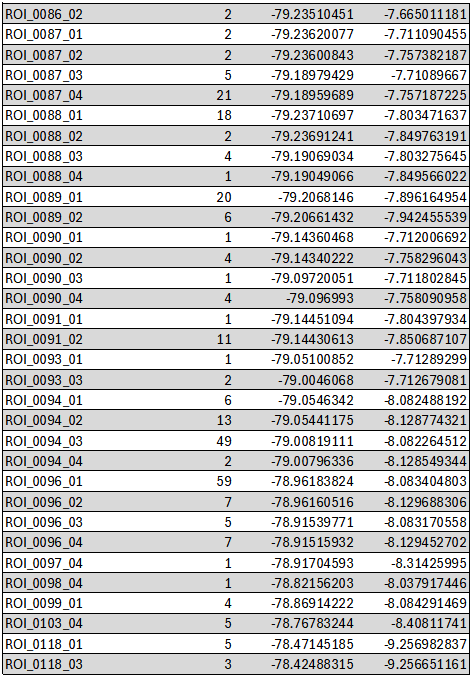
\includegraphics[width=0.9\textwidth]{img/8_capitulo6/ROI_2.png}
    \label{fig:figura_2}
\end{figure}
\begin{figure}[H]
    \centering
    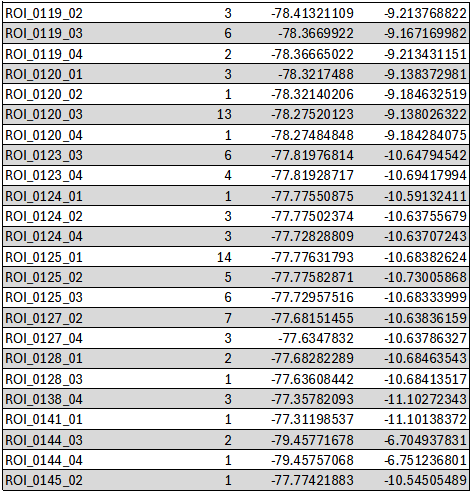
\includegraphics[width=0.9\textwidth]{img/8_capitulo6/ROI_3.png}
    \label{fig:figura_3}
    \begin{flushleft}
        \textit{Nota.} Elaboración propia.        
        \vspace{-\baselineskip}
    \end{flushleft}
\end{figure}